\documentclass[11pt]{article}

% Paquetes
%===================================================================================================

% Establecemos los márgenes
\usepackage[a4paper, margin=1in]{geometry}

% Separacion entre parrafos
\setlength{\parskip}{1em}

% Paquete para incluir codigo
\usepackage{listings}

% Paquete para incluir imagenes
\usepackage{graphicx}
\graphicspath{ {./Imagenes/} }

% Para fijar las imagenes en la posicion deseada
\usepackage{float}

% Para que el codigo acepte caracteres en utf8
\lstset{literate=
  {á}{{\'a}}1 {é}{{\'e}}1 {í}{{\'i}}1 {ó}{{\'o}}1 {ú}{{\'u}}1
  {Á}{{\'A}}1 {É}{{\'E}}1 {Í}{{\'I}}1 {Ó}{{\'O}}1 {Ú}{{\'U}}1
  {à}{{\`a}}1 {è}{{\`e}}1 {ì}{{\`i}}1 {ò}{{\`o}}1 {ù}{{\`u}}1
  {À}{{\`A}}1 {È}{{\'E}}1 {Ì}{{\`I}}1 {Ò}{{\`O}}1 {Ù}{{\`U}}1
  {ä}{{\"a}}1 {ë}{{\"e}}1 {ï}{{\"i}}1 {ö}{{\"o}}1 {ü}{{\"u}}1
  {Ä}{{\"A}}1 {Ë}{{\"E}}1 {Ï}{{\"I}}1 {Ö}{{\"O}}1 {Ü}{{\"U}}1
  {â}{{\^a}}1 {ê}{{\^e}}1 {î}{{\^i}}1 {ô}{{\^o}}1 {û}{{\^u}}1
  {Â}{{\^A}}1 {Ê}{{\^E}}1 {Î}{{\^I}}1 {Ô}{{\^O}}1 {Û}{{\^U}}1
  {ã}{{\~a}}1 {ẽ}{{\~e}}1 {ĩ}{{\~i}}1 {õ}{{\~o}}1 {ũ}{{\~u}}1
  {Ã}{{\~A}}1 {Ẽ}{{\~E}}1 {Ĩ}{{\~I}}1 {Õ}{{\~O}}1 {Ũ}{{\~U}}1
  {œ}{{\oe}}1 {Œ}{{\OE}}1 {æ}{{\ae}}1 {Æ}{{\AE}}1 {ß}{{\ss}}1
  {ű}{{\H{u}}}1 {Ű}{{\H{U}}}1 {ő}{{\H{o}}}1 {Ő}{{\H{O}}}1
  {ç}{{\c c}}1 {Ç}{{\c C}}1 {ø}{{\o}}1 {å}{{\r a}}1 {Å}{{\r A}}1
  {€}{{\euro}}1 {£}{{\pounds}}1 {«}{{\guillemotleft}}1
  {»}{{\guillemotright}}1 {ñ}{{\~n}}1 {Ñ}{{\~N}}1 {¿}{{?`}}1 {¡}{{!`}}1
}

% Para que no se salgan las lineas de codigo
% Para fijar una fuente que resalte
\lstset{breaklines=true, basicstyle=\ttfamily}


% Para que los metadatos que escribe latex esten en español
\usepackage[spanish]{babel}
\decimalpoint % Para que no se cambie el punto a la coma

% Para la bibliografia
% Sin esto, los enlaces de la bibliografia dan un error de compilacion
\usepackage{url}

% Para enlaces clickables
\usepackage{hyperref}

% Para mostrar graficas de dos imagenes, cada una con su caption, y con un caption comun
\usepackage{subcaption}

% Simbolo de los numeros reales
\usepackage{amssymb}

% Para que los codigos tengan una fuente distinta
\usepackage{courier}

\lstdefinestyle{CustomStyle}{
  language=Python,
  numbers=left,
  stepnumber=1,
  numbersep=10pt,
  tabsize=4,
  showspaces=false,
  showstringspaces=false
  basicstyle=\tiny\ttfamily,
}

% Para incluir tablas en csv
\usepackage{csvsimple}

% Para referenciar secciones usando el nombre de las secciones
\usepackage{nameref}

% Para enumerados dentro de enumerados
\usepackage{enumitem}

% Para mejores tablas
\usepackage{tabularx}

% Para poder tener el mismo identificador en dos tablas separadas
\usepackage{caption}

% Mostrar la página de las referencias en el indice del documento
\usepackage[nottoc,numbib]{tocbibind}

% Para mostrar las matrices
\usepackage{amsmath}

% Metadatos del documento
%===================================================================================================
\title{
    {Metaheurísticas - Proyecto Final}\\
    {\emph{Battle Royale Metaheuristic}}\\
    {\emph{Cec17 Competition}}
}

\author{
    {Sergio Quijano Rey - 72103503k}\\
    {sergioquijano@correo.ugr.es} \\
    {4º Doble Grado Ingeniería Informática y Matemáticas}
}

\date{\today}

% Separacion entre parrafos
\setlength{\parskip}{1em}

% Contenido del documento
%===================================================================================================
\begin{document}

% Portada del documento
\maketitle
\pagebreak

% Indice de contenidos
\tableofcontents

% Lista de figuras
\listoffigures

% Lista de tablas
\listoftables

\pagebreak
\section{Identificación del problema a resolver}

El problema a resolver consiste en realizar una propuesta de metaheurística original para problemas de codificación real. A partir de esta propuesta, realizaremos una implementación de dicha metaheurística original, y trabajaremos la competición \emph{Cec17}.

Para trabajar con dicha competición, usaremos el \emph{software} desarrollado por Daniel Molina, que se encuentra en \cite{daniel_repo:online}. En dicho repositorio encontramos el siguiente \emph{software}:

\begin{itemize}
    \item Librería escrita en \lstinline{C} que define las 31 funciones de \emph{fitness} que debemos optimizar, para las distintas dimensiones disponibles, así como otras funcionalidades
    \item Código \lstinline{python} para generar unas tablas \emph{Excel} que poder usar en \href{tacolab.org} para comparar con otros algoritmos de referencia
    \item Wrapper para \lstinline{Python}, con el que podemos acceder a todas las funciones definidas en la ya mencionada librería dinámica
\end{itemize}

En nuestro caso, como indicaron los profesores de la asignatura, por problemas con los tiempos de cómputo, trabajaremos con dimensión 10 y 30. Además, repetiremos por cada función y por cada dimensión, 10 ejecuciones distintas.

Por tanto, usamos un \emph{fork} de este repositorío para desarrollar nuestro trabajo, que se encuentra en \cite{repositorio:online}.

\pagebreak
\section{Descripción de la metaheurística} \label{descripcion}

\subsection{Propuesta original}

La metaheurística se basa en un género de videojuegos conocido como \emph{Battle Royale}. La dinámica de estos videojuegos se inspiran fuertemente en la serie de libros y posteriores películas `\emph{Los juegos del Hambre}', por lo que si el lector está familiarizado con estas novelas le será fácil seguir la siguiente explicación:

Una serie de jugadores (entre 50 y 100) se reparten a lo largo de un mapa. El objetivo es ser el último jugador vivo durante la partida. Para ello, tienen que seguir una serie de dinámicas durante la partida:

En primer lugar, al principio de la partida, los jugadores deben recolectar armas y otros recursos, porque todos los jugadores aparecen en el mapa sin equipación alguna. Esto puede verse reflejado en la metaheurística como una primera búsqueda local, muy suave, aplicada a las soluciones iniciales aleatorias

En segundo lugar, los jugadores deben matar y defenderse de los otros jugadores con los que se pueden encontrar a través del mapa. Para reflejar esto, si dos soluciones están muy cerca la una de la otra, estas dos soluciones compiten entre sí. El mejor jugador, que está mejor equipado, tiene una probabilidad alta de ganar la pelea, matando al otro jugador. Sin embargo, el peor jugador tiene una probabilidad pequeña de matar al mejor jugador (en el juego, puedes ir mejor equipado, pero perder el duelo por ser un jugador menos habilidoso). Soluciones muy cerca en el sentido en el que cierta distancia de los vectores que representan las dos soluciones estén por debajo de un valor dado.

En tercer lugar, a partir de cierto tiempo, el mapa se cierra incrementalmente sobre un área circular del mapa, cada vez más pequeña. Con esto se fomenta que los jugadores tengan que enfrentarse unos con otros, y potenciando que los jugadores mejor equipados y más habilidosos ganen sin tener que esperar demasiado tiempo a malos jugadores escondidos por el mapa.

Para representar esto en la metaheurística, a partir de cierta iteración, se realizarán eliminaciones de la población. A partir de este momento, cada cierto número de iteraciones, los $\lambda$ peores elementos de la población, son eliminados al quedar fuera del círculo.


La siguiente imagen, extraída de \cite{other_paper:paper}, ilustra de forma clara cuál es la mecánica del cierre del círculo:

\begin{figure}[H]
    \centering
    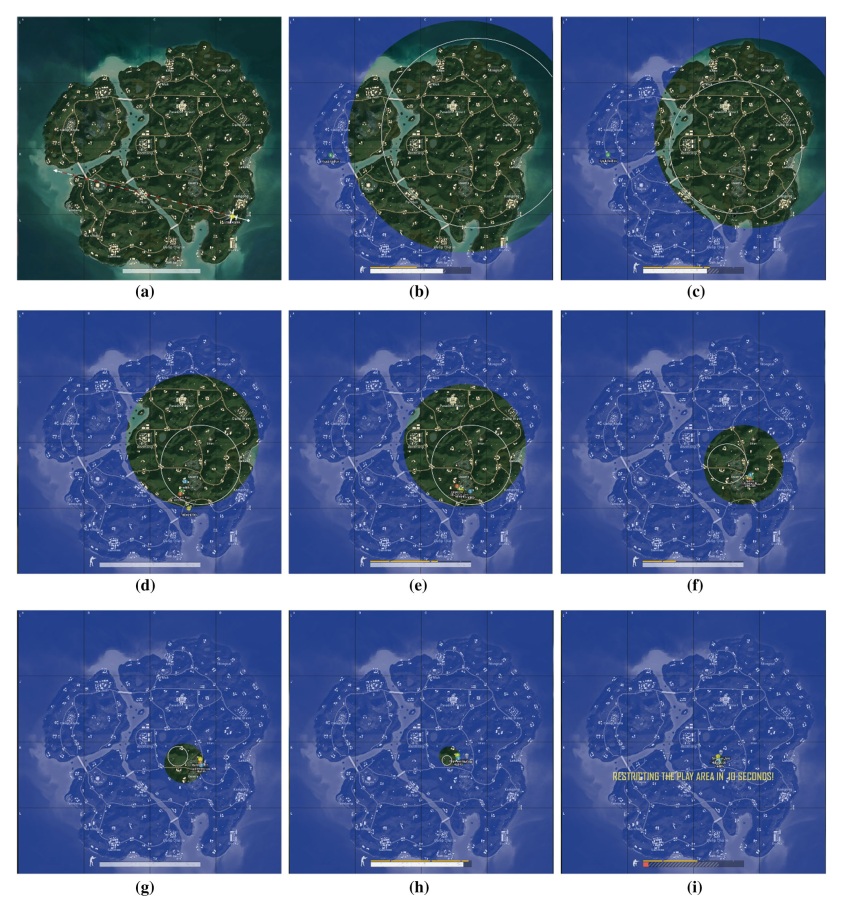
\includegraphics[width=0.6\textwidth]{cierre_circulo}
    \caption{Ilustración de la mecánica del cierre del círculo}
\end{figure}

Notar que la idea más natural para representar esta mecánica es cerrar el círculo sobre el espacio de búsqueda. Sin embargo, es una mala decisión, pues estamos restringiendo arbitrariamente soluciones en los bordes del espacio de búsqueda real, donde pueden encontrarse soluciones de buena calidad. Es por tanto que preferimos materializar la idea del círculo que se cierra sobre el fitness de los jugadores en referencia al mejor jugadr en vez de restringir el espacio de búsqueda.

En cuarto lugar, hay una cierta probabilidad de revivir si un jugador muere, aunque no es muy alta. Cuando un jugador revive, reaparece sin nada de lo que habías estado recolectando durante la partida. Se otorga un periodo de inmunidad en el que el jugador que ha revivido tiene que recolectar rápidamente recursos para ser competitivo contra jugadores que van más avanzados en la partida. Además, puede ser que reaparezcan fuera del círculo, luego deben lograr entrar al círculo en el tiempo de gracia

Por tanto, si un jugador muere, tiene una probabilidad dada (potencialmente baja) de revivir. Al revivir, pierde todos sus recursos. Esto se materializa en que se le asigna una solución aleatoria. En nomenclatura de nuestra metaheurística, reaparece en una posición aleatoria. Además, el periodo de gracia se materializa en que dispondrá de un número de iteraciones de una búsqueda local suave,  para intentar ser competitivo con el resto de soluciones que llevan toda la partida mejorando su fitness.

Decidimos también que, si un jugador muere contra el mejor jugador hasta el momento, revive siempre. Esto no se aplica cuando quedan menos de un número dado de jugadores (fase final de la partida)

Además de esto, consideramos algunos aspectos generales a todas las metaheurísticas vistas en clase:

En las distintas iteraciones, realizaremos una búsqueda local suave sobre las soluciones (para representar el movimiento por el mapa de los jugadores en la partida). Y como es habitual, partiremos de una población inicial aleatoria de jugadores. En el propio juego, los jugadores saltan desde el cielo eligiendo la posición inicial, y por tanto, podemos modelar este comportamiento como aleatorio.

\subsection{Modificaciones a la propuesta original}

Como era de esperar, esta propuesta original debe ser modificada ligeramente, pues algunas decisiones a nivel de ingeniería tienen más sentido. Las modificaciones que hemos considerado tras experimentar con la implementación de la metaheurística (implementación que se desarrollará en \emph{\ref{implementacion}. \nameref{implementacion}}) son las siguientes:

\begin{itemize}
    \item En un principio habíamos pensado en emplear la distancia euclídea para comprobar si dos jugadores estaban demasiado cerca. Sin embago, acabamos usando la distancia Manhattan porque es más rápida de computar. Esta distancia viene dada por $$\sum |w_i|$$ donde los coeficientes se definen como $$w := jugador_1 - jugador_2$$
    \item La mecánica de eliminar a los $\lambda$ peores jugadores en cada iteración, a partir de cierto momento, provoca que perdamos mucha variedad en la población prematuramente. En vez de eso, definimos un porcentaje que, a partir de un valor del radio del círculo $r$ por encima de $1.0$, que va descendiendo iteración tras iteración hasta llegar a $r = 1.0$. En cada iteración se eliminan los jugadores con \emph{fitness} más de $r$ veces peor que el \emph{fitness} de la mejor solución (recordad que estamos en un problema de minimización de las funciones objetivo)
    \item Tras hacer \emph{parameter tuning} en la sección \emph{\ref{tuning}. \nameref{tuning}}, la probabilidad de revivir acaba siendo 0.5, para nada es una probabilidad baja
    \item Por su poca relevancia, ignoramos la parte en la que comentamos que si un jugador muere contra el mejor jugador, forzosamente revive
\end{itemize}

\subsection{Trabajo existente}

En el \emph{paper} \cite{other_paper:paper}, se presenta una metaheurística basada también en este género de videojuegos. Sin embargo, en el proceso empleado para materializarla en una metaheurística concreta se toman decisiones completamente distintas a las que se presentan en este  trabajo. Por tanto, aunque la inspiración sea común, en la práctica las dos metaheurística son significativamente distintas.

En \cite{other_paper:paper}, cuando dos jugadores están cerca, se disparan entre ellos. Esto tiene dos efectos. El primero, el jugador que recibe el disparo aumenta en uno el contador de disparos recibido. Cuando el contador llega a un valor fijado, el jugador muere y resucita en un punto aleatorio del mapa. En segundo lugar, el jugador que recibe el disparo se mueve para evitar recibir más disparos. Este movimiento se hace en dirección hacia el mejor jugador.

Así, la propuesta \cite{other_paper:paper} considera una población de tamaño fijo, que no decrece como nuestra población, pues nuestra probabilidad de resucitar está por debajo de $1.0$. En segundo lugar, en las batallas no incluimos el mecanismo de movernos por el mapa. Usamos una búsqueda local suave para movernos por el mapa, en ningún momento queremos converger hacia la posición del mejor jugador.

\pagebreak
\section{Implementación de la metaheurística} \label{implementacion}

El desarrollo de esta metaheurística se ha realizado en \lstinline{python}, debido al rápido desarrollo que permite este lenguaje y la disponibilidad de \emph{wrappers} para el lenguaje gracias a \cite{daniel_repo:online}.

El proceso de instalación y ejecución del software se desarrolla en el \emph{Readme} del repositorio en el que tenemos alojado el código \cite{repositorio:online}, y por tanto no describimos de nuevo este proceso de instalación y ejecución necesario para trabajar con nuestra implementación.

Pasamos a comentar algunos aspectos clave de la implementación (no todo el código en general, que está a nuestro modo de ver lo suficientemente bien documentado como para que sea muy sencillo de leer).

\subsection{Pseudocódigo de la metaheurística}

Comentamos en primer lugar el pseudocódigo general de la metaheurística, que seguirá las ideas comentadas en \emph{\ref{descripcion}. \nameref{descripcion}}:

\begin{lstlisting}[language = python]
# Iniciamos una poblacion aleatoria
population = random_population(number of players)

# Condiciones para permanecer en la fase 1
phase1_condition = evals < max_evals and population.remaining_players() >= phase1_players_percentage
while pase1_condition:
    # Cada jugador se mueve por el mapa
    for player in population.players:
        player.soft_local_search()

    # Ronda de asesinatos entre jugadores cercanos
    # El primer jugador se elige aleatoriamente
    player1 = population.random_player

    # Se escoge un numero fijo de jugadores. Estos son los mas cercanos al player1
    players = n fijo jugadores mas cercanos a player1

    # Realizamos los asesinatos
    for player2 in players:
        # Los jugadores deben estar en un radio de vision
        if player1 no ve a player2:
            continue

        dead_player, resucitar = competir(player1, player2)
        if resucitar:
            # Aparece en una posicion aleatoria del mapa y tiene un periodo de gracia
            dead_player.respawn()
            dead_player.grace_time()


        # Si el jugador que muere es el player1, paramos
        if dead_player == player1 and resucitar == False:
            break

# Comienza la fase 2
circle_size = init_circle_size
while no se han consumido todas las iteraciones:
    # Los jugadores fuera del circulo mueren
    # Algunos pueden resucitar, haciendo player.respawn() y despues player.grace_time()
    population.kill_players_outside_circle()

    # Los jugadores se mueven algo
    for player in population.players:
        player.soft_local_search()


    # El circulo se cierra
    circle_size += circle_step

    # Si solo queda un jugador, paramos de iterar
    if len(population) == 1:
        break

# Devolvemos el mejor jugador
return population.get_best_player()
\end{lstlisting}

La búsqueda local suave utilizada se describe en el siguiente pseudocódigo:

\begin{lstlisting}
def soft_local_search(self):
    best_player = self

    for _ in 0..tries_in_local_search:
        # Se selecciona la coordenada y el valor de variacion de forma aleatoria
        position = random(0, len(self.position))
        delta = random(step_size, step_size)

        # Modificamos la posicion
        new_position = self.position.copy()
        new_position[position] = new_position[position] + delta

        # Generamos el nuevo jugador
        new_player = None
        new_player = Player(self.dimension, new_position)

        # Si el jugador no es valido, lo ignoramos
        if new_player.is_valid == False:
            continue

        # Comprobamos si es mejor que el mejor jugador hasta el momento
        new_pla_fit = new_player.fitness()
        if new_player.fitness() < best_player.fitness():
            best_player = new_player


    # Hacemos el cambio mas optimo
    self = best_player
\end{lstlisting}


Con este pseudocódigo en mente, podemos describir algunos detalles relevantes de la implementación.

\subsection{Clase \lstinline{Config}}

La clase \lstinline{Config} centraliza todos los parámetros que hemos fijado en nuestra metaheurística. Los atributos estáticos hace que sea fácil acceder a parámetros comunes en distintas partes del código sin una penalización en tiempos de ejecución aparentemente relevante.

Además, como se hace en la función \lstinline{parameter_tuning} de \lstinline{main.py}, podemos modificar estos atributos estáticos para ver cómo afecta esto al rendimiento de nuestra metaheurística.

\subsection{Clase \lstinline{EvalsCounter}}

Esta clase se implementa con el uso del patrón \emph{Singleton}. Su objetivo es centralizar la cuenta de evaluaciones del \emph{fitness} consumidas hasta el momento, sin tener que pasar a todos los métodos una parámetro adicional.

Sin embargo, sospechamos que esto sí que puede introducir una penalización en tiempo de ejecución. Pero al estar escribiendo un primer prototipo, vale más la pena trabajar con un código mas sencillo en el que es más rápido realizar cambios sobre la marcha (como hemos tenido que realizar, al no tener una metaheurística ya desarrollado con un funcionamiento bueno asegurado).

En una versión mejorada en la que los tiempos de ejecución sean más críticos, evitar este patrón \emph{Singleton} es obligado.

\subsection{Clase \lstinline{Player}}

Define un jugador. Principalmente, viene dado por las coordenadas en las que se encuentra, que vienen dadas por \lstinline{self.position}.

Por motivos de eficiencia, \emph{cacheamos} el valor del \emph{fitness}, para evitar desperdiciar evaluaciones del \emph{fitness}. Del mismo modo, en la propia lógica que maneja la cache, usamos el \emph{Singleton} que ya hemos comentado para llevar la cuenta de todas las evaluaciones del \emph{fitness} consumidas.

\subsection{Clase \lstinline{Population}}

Representa al conjunto de jugadores. Permite inicializar poblaciones de jugadores aleatorias, aplicar búsquedas locales sobre todos los jugadores de la población, matar a los jugadores fuera del círculo, tomar al mejor jugador de la población, aplicar periodos de gracia a jugadores resucitados, \ldots

\subsection{Clase \lstinline{BattleRoyale}}

Representa el código de alto nivel de la metaheurística, principalmente lanzando el código necesario para la primera y segunda fase. Usa los métodos que la clase \lstinline{Population} ofrece para realizar operaciones sobre toda la población ya comentadas, y para realizar las comprobaciones que determinan en qué fase de la metaheurística nos encontramos.

El método más importante es \lstinline{run_game}, que permite lanzar la ejecución de la metaheurística.

\subsection{\emph{Parameter Tuning}} \label{tuning}

Si se consulta la clase \lstinline{Config}, se pueden consultar todos los parámetros libre que hemos tenido que establecer en nuestra metaheurística. A continuación se da una breve descripción de cada uno de ellos:

\begin{itemize}
    \item \lstinline{lower_range}, \lstinline{upper_range}: el rango de las funciones reales con las que trabajamos. En cada coordenada, trabajamos con el rango $[-100, 100]$
    \item \lstinline{number_of_players}: número de jugadores iniciales cuando comienza una partida
    \item \lstinline{ev_per_dimension}: evaluaciones del fitness por cada dimensión del problema. Es un valor fijado a $10.000$
    \item \lstinline{phase1_percentage}: porcentaje de evaluaciones máximas que reservamos para la primera fase de la partida
    \item \lstinline{phase1_players_percentage}: porcentaje mínimo de jugadores con los que puede finalizar la primera fase de la partida
    \item \lstinline{tries_in_local_search}: intentos que se pueden emplear en la búsqueda local suave
    \item \lstinline{step_size}: tamaño de salto para la búsqueda local
    \item \lstinline{player_radius_vision_per_dimension}: radio de visión de los jugadores
    \item \lstinline{players_to_compete}: número de jugadores con los que compite el jugador aleatorio escogido
    \item \lstinline{best_player_survives_prob}: probabilidad de que el mejor jugador sobreviva en una batalla
    \item \lstinline{resurrect_prob}: probabilidad de resurrección
    \item \lstinline{number_of_grace_soft_local_search}: número de búsquedas locales suaves que se usan cuando un jugador revive como tiempo de gracia
    \item \lstinline{init_circle_size}: tamaño inicial del círculo
    \item \lstinline{circle_step}: controla el cerrado del círculo
\end{itemize}

Por tanto, debemos buscar un método para fijar unos valores de estos parámetros, lo más óptimos posibles empleando un tiempo de computación razonable. El proceso ideal sería emplear \emph{Grid Search} sobre todas las combinaciones de los parámetros libres que queramos explorar. Sin embargo, esto no es factible en un tiempo razonable, y por tanto empleamos otro enfoque más rápido aunque subóptimo.

Empleamos una combinación de búsqueda binaria con la técnica \emph{Coordinate Descent}. Elegimos un parámetro libre a optimizar. Realizamos sucesivas búsquedas binarias hasta encontrar un valor óptimo para el parámetro. Tras esto, realizamos el mismo proceso iterativamente con las parámetros libres restantes.

Además, solo hacemos esta búsqueda en dimensión 10, para acelerar el proceso, a pesar de que este procedimiento sea subóptimo.

Este proceso lo realizamos de forma manual usando la función \lstinline{parameter_tuning} del fichero \lstinline{main.py}. Los resultados en bruto de este proceso se muestran en el fichero \lstinline{parameter_tuning/parameter_tuning_results.txt}. Resumimos los resultados en las siguientes tablas, comenzando por el número de jugadores:

\begin{table}[H]
    \centering
    \resizebox{1.1\textwidth}{!}{
    \begin{tabular}{|c|c|c|c|c|}
        \hline
        \textbf{Primer parámetro} & \textbf{Segundo parámetro} & \textbf{Error del primer parámetro} & \textbf{Error del segundo parámetro} & \textbf{Error primero / Error segundo} \\
        \hline
        5000 & 10.000 & 659477824.1690311 & 285275478.41262203 & 2.12922252252212 \\
        10.000 & 20.000 & 188325303.46050686 & 169032537.0438895 & 1.187489601248911 \\
        20.000 & 25.000 & 419574922.2396657 &  278099949.5320168 & 1.089308035166435 \\
        \hline
    \end{tabular}}
    \caption{\emph{Parameter Tuning} para el número de jugadores}
\end{table}

A pesar de que los mejores resultados los obtengamos con 25.000 jugadores, elegimos usar 20.000 jugadores, porque los tiempos de ejecución son demasiado lentos con 25.000 jugadores. Por el mismo motivo, paramos la búsqueda aunque valores más altos sean prometedores.

A continuación, exploramos la probabilida de resucitar:

\begin{table}[H]
    \centering
    \resizebox{1.1\textwidth}{!}{
    \begin{tabular}{|c|c|c|c|c|}
        \hline
        \textbf{Primer parámetro} & \textbf{Segundo parámetro} & \textbf{Error del primer parámetro} & \textbf{Error del segundo parámetro} & \textbf{Error primero / Error segundo} \\
        \hline
        0.05 & 0.1 & 419574922.2396657 & 195545700.25415954 & 1.1796652597282404 \\
        0.1 & 0.5 & 530618675.60314316 & 238315604.57736704 & 1.357938844000634 \\
        0.5 & 0.25 & 57071508.32941685 & 275490531.32538956 & 1.0400957207903052 \\
        \hline
    \end{tabular}}
    \caption{\emph{Parameter Tuning} para la probabilidad de resucitar}
\end{table}

Aunque probabilidades por encima de 0.5 parezcan prometedoras, pues no paramos de mejorar, no queremos emplear probabilidades por encima de 0.5. De lo contrario, estaríamos realizando demasiadas búsquedas locales, restándole protagonismo a los otros mecanismos de nuestra metaheurística. Queremos que la búsqueda local sea un componente secundario que permita a los jugadores moverse por el mapa. Cuando realicemos la hibridación, la búsqueda local pasará a tener un papel principal.

Hecho esto, pasamos a ajustar el parámetro del radio de visión:

\begin{table}[H]
    \centering
    \resizebox{1.1\textwidth}{!}{
    \begin{tabular}{|c|c|c|c|c|c|}
        \hline
        \textbf{Primer parámetro} & \textbf{Segundo parámetro} & \textbf{Dimensión} & \textbf{Error del primer parámetro} & \textbf{Error del segundo parámetro} & \textbf{Error primero / Error segundo} \\
        \hline
        50 & 100 & 10 &  145468977.6843304 & 199935070.89682162 & 0.8521445003322603 \\
        50 & 75 & 10 & 145468977.6843304 & 199767035.44570535 & 0.8980227918235176 \\
        50 & 25 & 10 & 145468977.6843304 & 199309400.0598218 & 1.672495760214323 \\
        50 & 25 & 30 & 9.063796890289635e+40 & 2.463649041371674e+41 & 0.9437658215205048 \\
        \hline
    \end{tabular}}
    \caption{\emph{Parameter Tuning} para el radio de visión}
\end{table}

Por el comportamiento que se muestra en las tablas, tomamos 50 como valor para el parámetro.

El resto de parámetros los fijamos según la intuición que tenemos sobre el problema que estamos tratando. De nuevo, todos los valores empleados para los parámetros se pueden consultar cómodamente en la clase \lstinline{Config}

Notar también que cuando hagamos la hibridación, introduciremos nuevos parámetros. En \emph{\ref{tuning_hib}. \nameref{tuning_hib}}, realizaremos de nuevo este proceso con los parámetros de la metaheurística hibridada.

\pagebreak
\section{Resultados de la metaheurística} \label{resultados}

Usaremos el software proporcionado por Daniel Molina \cite{daniel_repo:online} para realizar las comparaciones. En primer lugar, usaremos el siguiente \emph{script} de \lstinline{Python} para generar los ficheros \emph{Excel}:

\begin{lstlisting}[language=Bash]
$ python3 ./src/extract.py results_battle_royale_standar/
\end{lstlisting}

Usando la web \url{https://tacolab.org}, desarrollada también por Daniel Molina, podemos comparar nuestros resultados almacenados en ficheros \emph{Excel} con otras metaheurísticas.

Como metaheurísticas de comparación, emplearemos \emph{differential evolution} y \emph{particle swarm optimization}. Ambas Metaheurísticas han sido vistas en la asignatura y dan muy buenos resultados, por lo que las consideramos adecuadas a la hora de comparar nuestros resultados.


\subsection{Resultados en dimensión 10}

\begin{table}[H]
\centering
\begin{tabular}{|c|c|c|c|}
\hline
\textbf{Función} & \textbf{Battle Royale} &         \textbf{DE} &        \textbf{PSO} \\
\hline
F01  &     3.940e+09 &  0.000e+00 &  5.255e+07 \\
F02  &     4.716e+09 &  0.000e+00 &  1.000e+00 \\
F03  &     9.935e+03 &  0.000e+00 &  1.989e+03 \\
F04  &     2.743e+02 &  1.105e-04 &  4.684e+01 \\
F05  &     7.338e+01 &  1.151e+02 &  3.212e+01 \\
F06  &     4.078e+01 &  3.460e+01 &  1.001e+01 \\
F07  &     1.814e+02 &  3.848e+01 &  4.275e+01 \\
F08  &     6.805e+01 &  2.983e+01 &  2.203e+01 \\
F09  &     8.848e+02 &  1.938e+02 &  5.686e+01 \\
F10  &     1.418e+03 &  3.597e+02 &  1.077e+03 \\
F11  &     3.965e+02 &  1.942e-02 &  3.843e+01 \\
F12  &     9.295e+07 &  4.931e+00 &  2.517e+06 \\
F13  &     1.991e+05 &  5.988e+00 &  8.409e+03 \\
F14  &     4.402e+02 &  5.240e-02 &  9.993e+01 \\
F15  &     4.417e+03 &  6.060e-02 &  2.066e+03 \\
F16  &     3.031e+02 &  4.561e+02 &  1.415e+02 \\
F17  &     1.561e+02 &  2.350e+01 &  6.497e+01 \\
F18  &     8.299e+05 &  3.630e-02 &  1.484e+04 \\
F19  &     8.058e+03 &  5.192e-03 &  3.220e+03 \\
F20  &     1.393e+02 &  3.837e+02 &  8.444e+01 \\
F21  &     1.577e+02 &  1.889e+02 &  1.320e+02 \\
F22  &     3.186e+02 &  1.005e+02 &  7.740e+01 \\
F23  &     3.974e+02 &  8.098e+02 &  3.304e+02 \\
F24  &     3.533e+02 &  1.000e+02 &  1.810e+02 \\
F25  &     6.516e+02 &  4.040e+02 &  4.478e+02 \\
F26  &     8.484e+02 &  2.706e+02 &  3.729e+02 \\
F27  &     4.587e+02 &  3.897e+02 &  4.134e+02 \\
F28  &     6.182e+02 &  3.517e+02 &  4.698e+02 \\
F29  &     4.298e+02 &  2.375e+02 &  3.193e+02 \\
F30  &     4.042e+06 &  8.051e+04 &  6.352e+05 \\
Best &             0 &         21 &          9 \\
\hline
\end{tabular}
    \caption{Media del error tras el 100\% de las evaluaciones y cuenta del mejor algoritmo}
\end{table}

A la vista de esta tabla, observando directamente la última columna, vemos que nuestro algoritmo nunca gana a \emph{DE} ni a \emph{PSO}.

En muchas ocasiones, obtenemos resultados órdenes de magnitud por encima del segundo peor resultado. Por ejemplo, para $F30$, obtenemos un resultado 10 veces peor que el segundo peor. En $f01$, obenemos un resultado 100 veces peor que el segundo peor. Por tanto, concluimos que estamos obteniendo resultados significativamente peores que los obtenidos por las metaheurísticas de comparación.

En la siguiente tabla, mostramos el ranking sobre las distintas funciones:

\begin{table}[H]
\centering
\begin{tabular}{|c|c|c|c|}
\hline
\textbf{Función} & \textbf{Battle Royale} &         \textbf{DE} &        \textbf{PSO} \\
\hline
F01  &             3 &      1 &      2 \\
F02  &             3 &      1 &      2 \\
F03  &             3 &      1 &      2 \\
F04  &             3 &      1 &      2 \\
F05  &             2 &      3 &      1 \\
F06  &             3 &      2 &      1 \\
F07  &             3 &      1 &      2 \\
F08  &             3 &      2 &      1 \\
F09  &             3 &      2 &      1 \\
F10  &             3 &      1 &      2 \\
F11  &             3 &      1 &      2 \\
F12  &             3 &      1 &      2 \\
F13  &             3 &      1 &      2 \\
F14  &             3 &      1 &      2 \\
F15  &             3 &      1 &      2 \\
F16  &             2 &      3 &      1 \\
F17  &             3 &      1 &      2 \\
F18  &             3 &      1 &      2 \\
F19  &             3 &      1 &      2 \\
F20  &             2 &      3 &      1 \\
F21  &             2 &      3 &      1 \\
F22  &             3 &      2 &      1 \\
F23  &             2 &      3 &      1 \\
F24  &             3 &      1 &      2 \\
F25  &             3 &      1 &      2 \\
F26  &             3 &      1 &      2 \\
F27  &             3 &      1 &      2 \\
F28  &             3 &      1 &      2 \\
F29  &             3 &      1 &      2 \\
F30  &             3 &      1 &      2 \\
Mean &         2.833 &  1.467 &  1.700 \\
\hline
\end{tabular}
    \caption{Ranking de los tres algoritmos y media en el ranking}
\end{table}

Vemos que en algunas funciones concretas, nuestro algoritmo consigue posicionarse como segundo, por encima de \emph{DE}. Sin embargo, el valor medio indica que tenemos la peor metaheurística consistentemente sobre las distintas funciones.

Mostramos ahora cómo avanza este ranking según el porcentaje de las evaluaciones del \emph{fitness} que se han consumido:

\begin{table}[H]
\centering
\resizebox{\textwidth}{!}{
\begin{tabular}{|c|c|c|c|c|c|c|c|c|c|c|c|c|c|c|}
\hline
\textbf{Metaheurística} &       1   &       2   &       3   &       5   &       10  &       20  &       30  &       40  &       50  &       60  &       70  &       80  &       90  &       100 \\
\hline
BATTLE ROYALE &  2.133333 &  2.166667 &  2.166667 &  2.666667 &  2.800000 &  2.833333 &  2.833333 &  2.833333 &  2.833333 &  2.833333 &  2.833333 &  2.833333 &  2.833333 &  2.833333 \\
DE            &  2.700000 &  2.666667 &  2.666667 &  1.900000 &  1.433333 &  1.400000 &  1.400000 &  1.400000 &  1.433333 &  1.466667 &  1.466667 &  1.466667 &  1.466667 &  1.466667 \\
PSO           &  1.166667 &  1.166667 &  1.166667 &  1.433333 &  1.766667 &  1.766667 &  1.766667 &  1.766667 &  1.733333 &  1.700000 &  1.700000 &  1.700000 &  1.700000 &  1.700000 \\
\hline
\end{tabular}}
    \caption{Ranking según el avance del porcentaje de evaluaciones consumidas}
    \label{ranking_1}
\end{table}

Si nos fijamos en como avanza el ranking de nuestra metaheurística a lo largo del porcentaje de las evaluaciones del \emph{fitness}, podemos ver que a partir del 10\% de las evaluaciones del fitness empeoramos significativamente nuestro ranking, sin empeorar apenas a partir de este momento.

Esto nos hace sospechar que nuestra metaheurística tiene demasiada exploración (pues no funciona mal en porcentajes bajos de evaluaciones), pero tiene poca explotación (pues empeora en fases avanzadas del porcentaje de evaluaciones).

\subsection{Resultados en dimensión 30}

\begin{table}[H]
\centering
\begin{tabular}{|c|c|c|c|}
\hline
\textbf{Función} & \textbf{Battle Royale} &         \textbf{DE} &        \textbf{PSO} \\
\hline
F01  &     6.627e+10 &  4.909e+04 &  4.175e+09 \\
F02  &     5.012e+43 &  1.309e+19 &  1.000e+00 \\
F03  &     1.109e+05 &  3.481e+03 &  5.453e+04 \\
F04  &     1.336e+04 &  8.430e+01 &  1.183e+03 \\
F05  &     4.663e+02 &  2.015e+02 &  2.170e+02 \\
F06  &     9.448e+01 &  6.320e+00 &  3.694e+01 \\
F07  &     1.760e+03 &  2.334e+02 &  3.596e+02 \\
F08  &     4.211e+02 &  1.894e+02 &  1.745e+02 \\
F09  &     1.479e+04 &  6.530e+01 &  2.842e+03 \\
F10  &     7.637e+03 &  3.764e+03 &  6.938e+03 \\
F11  &     9.194e+03 &  7.958e+01 &  1.207e+03 \\
F12  &     8.307e+09 &  3.258e+05 &  3.586e+08 \\
F13  &     4.079e+09 &  1.536e+02 &  4.508e+07 \\
F14  &     8.678e+05 &  7.100e+01 &  3.059e+05 \\
F15  &     4.826e+08 &  6.256e+01 &  2.737e+05 \\
F16  &     3.329e+03 &  1.319e+03 &  1.568e+03 \\
F17  &     1.545e+03 &  4.809e+02 &  4.725e+02 \\
F18  &     1.385e+07 &  6.122e+01 &  2.170e+06 \\
F19  &     5.531e+08 &  3.572e+01 &  1.260e+06 \\
F20  &     9.440e+02 &  2.751e+02 &  4.621e+02 \\
F21  &     6.119e+02 &  3.255e+02 &  4.113e+02 \\
F22  &     7.238e+03 &  1.002e+02 &  1.027e+03 \\
F23  &     1.070e+03 &  5.346e+02 &  6.404e+02 \\
F24  &     1.160e+03 &  6.059e+02 &  7.095e+02 \\
F25  &     5.187e+03 &  3.870e+02 &  6.864e+02 \\
F26  &     7.617e+03 &  4.038e+02 &  3.369e+03 \\
F27  &     1.333e+03 &  4.925e+02 &  8.068e+02 \\
F28  &     4.161e+03 &  3.943e+02 &  1.105e+03 \\
F29  &     3.048e+03 &  1.025e+03 &  1.409e+03 \\
F30  &     5.775e+08 &  3.657e+03 &  1.359e+07 \\
Best &             0 &         27 &          3 \\
\hline
\end{tabular}
    \caption{Media del error tras el 100\% de las evaluaciones y cuenta del mejor algoritmo}
\end{table}

De nuevo, obtenemos unos resultados malos en comparación a las dos metaheurísticas consideradas. Y de nuevo, tenemos resultados órdenes de magnitud superiores. Del mismo modo, mostramos los rankings:

\begin{table}[H]
\centering
\begin{tabular}{|c|c|c|c|}
\hline
\textbf{Función} & \textbf{Battle Royale} &         \textbf{DE} &        \textbf{PSO} \\
\hline
F01  &             3 &      1 &      2 \\
F02  &             3 &      2 &      1 \\
F03  &             3 &      1 &      2 \\
F04  &             3 &      1 &      2 \\
F05  &             3 &      1 &      2 \\
F06  &             3 &      1 &      2 \\
F07  &             3 &      1 &      2 \\
F08  &             3 &      2 &      1 \\
F09  &             3 &      1 &      2 \\
F10  &             3 &      1 &      2 \\
F11  &             3 &      1 &      2 \\
F12  &             3 &      1 &      2 \\
F13  &             3 &      1 &      2 \\
F14  &             3 &      1 &      2 \\
F15  &             3 &      1 &      2 \\
F16  &             3 &      1 &      2 \\
F17  &             3 &      2 &      1 \\
F18  &             3 &      1 &      2 \\
F19  &             3 &      1 &      2 \\
F20  &             3 &      1 &      2 \\
F21  &             3 &      1 &      2 \\
F22  &             3 &      1 &      2 \\
F23  &             3 &      1 &      2 \\
F24  &             3 &      1 &      2 \\
F25  &             3 &      1 &      2 \\
F26  &             3 &      1 &      2 \\
F27  &             3 &      1 &      2 \\
F28  &             3 &      1 &      2 \\
F29  &             3 &      1 &      2 \\
F30  &             3 &      1 &      2 \\
Mean &         3.000 &  1.100 &  1.900 \\
\hline
\end{tabular}
    \caption{Ranking de los tres algoritmos y media en el ranking}
\end{table}

En esta dimensión, los resultados han sido todavía peores, no logrando en ninguna funcion alcanzar el puesto segundo. Podemos suponer, por tanto, que nuestra metaheurística funciona peor cuantas más dimensiones consideremos. Del mismo modo, mostramos el ranking según avanzan los porcentajes de evaluación del fitness:


\begin{table}[H]
\centering
\resizebox{\textwidth}{!}{
\begin{tabular}{|c|c|c|c|c|c|c|c|c|c|c|c|c|c|c|}
\hline
\textbf{Metaheurística} &       1   &       2   &       3   &       5   &       10  &       20  &       30  &       40  &       50  &       60  &       70  &       80  &       90  &       100 \\
\hline
BATTLE ROYALE &  2.366667 &  2.400000 &  2.666667 &  3.000000 &  3.000000 &  3.0 &  3.000000 &  3.000000 &  3.000000 &  3.000000 &  3.0 &  3.0 &  3.0 &  3.0 \\
DE            &  2.500000 &  2.466667 &  2.133333 &  1.266667 &  1.133333 &  1.1 &  1.066667 &  1.066667 &  1.066667 &  1.066667 &  1.1 &  1.1 &  1.1 &  1.1 \\
PSO           &  1.133333 &  1.133333 &  1.200000 &  1.733333 &  1.866667 &  1.9 &  1.933333 &  1.933333 &  1.933333 &  1.933333 &  1.9 &  1.9 &  1.9 &  1.9 \\
\hline
\end{tabular}}
    \caption{Ranking según el avance del porcentaje de evaluaciones consumidas}
    \label{ranking_2}
\end{table}

En esta dimensión, nuestra metaheurística deja de usar de forma efectiva las evaluaciones del \emph{fitness}, respecto a las otras dos metaheurísticas de comparación, mucho más rápido. A partir del 5\% de las evaluaciones, dejamos de ser relevantes.

\subsection{Conclusiones}

Como se muestra en las tablas \emph{\ref{ranking_1}. \nameref{ranking_1}} y \emph{\ref{ranking_2}. \nameref{ranking_2}}, no estamos aprovechando las evaluaciones del \emph{fitness} a partir de cierto porcentaje de forma tan efectiva como lo hacen \emph{DE} y \emph{PSO}. Sospechamos que necesitamos introducir mayor explotación para poder ser competitivos, pues de momento tenemos una metaheurística que diversifica demasiado. Esto se visibiliza en resultados no muy malos en porcentajes bajos de las evaluaciones del \emph{fitness}, y con resultados que empeoran relativamente a las otras dos metaheurísticas con el paso de las evaluaciones del \emph{fitness}.

Además, viendo estos resultados, nos damos cuenta de que al final de la fase dos de la metaheurística, devolvemos el mejor jugador directamente. Pueden quedar muchas evaluaciones del \emph{fitness} sin consumir, pues la fase dos puede acabar si solo queda un jugador vivo, aunque queden maś evaluaciones del \emph{fitness}. Por tanto, y como comentaremos en \emph{\ref{hibridacion}. \nameref{hibridacion}}, resolveremos este problema introduciendo una búsqueda local fuerte sobre el mejor jugador hasta agotar las evaluaciones.

Notar que podríamos haber corregido este inconveniente empleando búsquedas locales suaves hasta agotar las iteraciones. Sin embargo, el proceso de lanzar todos los casos tardó aproximadamente unas seis horas, y por tanto, no nos es factible volver a repetir estos cómputos.

Por tanto, queda claro que necesitamos introducir de forma efectiva un mecanismo que intensifique las soluciones, puesto que tenemos demasiada exploración. Nos encargaremos de esto en la hibridación del algoritmo.

\pagebreak
\section{Hibridación con la búsqueda local \emph{Solis West}} \label{hibridacion}

\subsection{Mecanismo de hibridación}

Para la hibridación usaremos la búsqueda local proporcionada por Daniel Molina en su repositorio \cite{daniel_repo:online}. En su código nos ha proporcionado la búsqueda \emph{Solis West} que usaremos como búsqueda local fuerte.

Para la hibridación, la primera idea que consideramos es aplicar alguna de las hibridaciones vistas en las prácticas de la asignatura. Por ejemplo, cada cierto número de iteraciones, realizar la búsqueda local fuerte sobre toda la población, sobre un porcentaje aleatorio de la población o sobre el mejor porcentaje de la población.

Sin embargo, dado el carácter exploratorio de este trabajo, decidimos introducir la búsqueda local fuerte en alguna de las componentes de nuestra metaheurística original. En concreto, pensamos que tiene interés introducir la hibridación sobre el mecanismo de resurrección de jugadores, pues como ya se ha visto, es el mecanismo principal del que dispone la metaheurística para introducir diversidad en la población. Y por tanto, es el lugar indicado donde vamos a buscar un equilibrio entre exploración (dada por la resurrección) y explotación (dada por la búsqueda local fuerte en el periodo de gracia).

Así que cuando un jugador muere, emplea la búsqueda local fuerte durante el periodo de gracia, buscando ser tan competitivo como el resto de jugadores.

Además, como ya hemos comentado en \emph{\ref{resultados}. \nameref{resultados}}, no estamos usando las evaluaciones del fitness que nos sobran tras finalizar la fase dos. Este es un buen punto en el que aplicar una búsqueda local fuerte sobre el mejor jugador de la población que vamos a devolver, para introducir más explotación en nuestra metaheurística.

\subsection{Implementación}

En la implementación de la clase \lstinline{BattleRoyale}, tenemos un atributo \lstinline{memetic} evaluado a \lstinline{False}. En la implementación de \lstinline{BattleRoyale.run_game()}, ya introducimos la lógica que hace que empleemos las búsquedas locales fuertes al resucitar y al acabar la fase 2. Así que lo que queda por hacer es crear una clase \lstinline{BattleRoyaleMemetic} que herede de \lstinline{BattleRoyale} y que únicamente modifique el inicializador para que \lstinline{memetic == True}.


\subsection{Parameter Tuning para la hibridación} \label{tuning_hib}

Los nuevos parámetros con los que tenemos que trabajar son:

\begin{itemize}
    \item \lstinline{max_evals_hard_local_search}: máximo de evaluaciones que permitimos por cada búsqueda local fuerte
    \item \lstinline{delta}: valor que controlar el comportamiento de la búsqueda \emph{Solis West}
\end{itemize}

Se recomienda que $\delta \in [0.1, 0.2]$, así que fijamos $\delta = 0.15$. Para el máximo de evaluaciones por cada búsqueda local, repetimos el proceso de \emph{parameter tuning}:

\begin{table}[H]
    \centering
    \resizebox{1.1\textwidth}{!}{
    \begin{tabular}{|c|c|c|c|c|}
        \hline
        \textbf{Primer parámetro} & \textbf{Segundo parámetro} & \textbf{Error del primer parámetro} & \textbf{Error del segundo parámetro} & \textbf{Error primero / Error segundo} \\
        \hline
        100 & 200 & 57071508.32941685 & 21936177.06833397 & 704.8020373037883 \\
        200 & 500 & 432924725.45316225 & 38147478.32365207 & 252.93678368043257 \\
        500 & 375 & 18104481.526603617 & 79681777.65233472 & 1.3939502593398763 \\
        \hline
    \end{tabular}}
    \caption{\emph{Parameter Tuning} para el máximo de evaluaciones por cada búsqueda local fuerte}
\end{table}

Así que empleamos como mucho 375 evaluaciones del \emph{fitness} por cada búsqueda local fuerte que empleemos.

\pagebreak
\section{Resultados de la hibridación}

\subsection{Resultados en dimensión 10}
\subsection{Resultados en dimensión 30}
\subsection{Conclusiones}

\pagebreak
\section{Propuesta de mejoras} \label{mejoras}

Con todo este trabajo, podemos proponer algunas mejoras que se siguen de los problemas que hemos encontrando en el desarrollo de esta práctica.

En primer lugar, para una futura implementación, es necesario abandonar el uso del patrón \emph{Singleton}. En primer lugar, porque tiene un efecto negativo sobre los tiempos de cómputo. En segundo lugar, por todos los problemas que puede introducir a nivel de diseño, como por ejemplo problemas a la hora de escribir \emph{testing} al código. Cabe resaltar que el uso actual que hacemos del patrón no permite que introduzcamos paralelismo a la metaheurística, lo que sería muy interesante porque la base poblacional puede explotar en varias partes dicho paralelismo.

En segundo lugar, hemos desarrollado una metaheurística que depende de demasiados parámetros. A la hora de aplicar la metaheurística de forma eficiente sobre un problema nuevo, debemos hacer \emph{parameter tuning} de forma efectiva para lograr buenos resultados. Con tantos parámetros libre, una técnica como \emph{Grid Search} supone unos tiempos de cómputo no razonables. Por tanto, se proponen dos posibles soluciones a este problema:

\begin{itemize}
    \item Realizar un estudio de los parámetros óptimos para distintos problemas, e intentar fijar el mayor número de parámetros libres posibles (aquellos con baja variabilidad entre distintos problemas). Con ello, solo se tendría que realizar \emph{parameter tuning} sobre una conjunto reducido de parámetros libres
    \item De forma alternativa o adicional, introducir parámetros adaptativos, mucho más flexibles a la hora de trabajar con problemas de distintas carácterísticas. Estos parámetros adaptativos dependerían también de algunos parámetros, pero definitivamente de muchos menos parámetros que los que se especifican en nuestra metaheurística
\end{itemize}

\pagebreak

% Bibliografia
\bibliography{./References}
\bibliographystyle{acm}

\end{document}
